% \documentclass[twocolumn]{article}
\documentclass{article}
\usepackage{graphicx}
% \usepackage[T1]{fontenc}
% \usepackage{charter}
\usepackage{authblk}
\usepackage{hyperref}
\usepackage{natbib}
\usepackage{array}
\usepackage{amsmath}
% \usepackage{float}


\setlength{\marginparwidth}{2cm}
\usepackage{todonotes}

\title{Style transfer with large language models}
\author[1]{Guillem Chillon}
\author[2]{Jordan Matelsky}
\author[3]{Zixuan Bian}
\affil[1]{guillemc@seas.upenn.edu}
\affil[2]{matelsky@upenn.edu}
\affil[3]{bianzx@seas.upenn.edu}
\date{May 2025}

\begin{document}

\maketitle

\begin{abstract}
% Context:
Style transfer in text generation is a challenging problem due to the difficulty of altering style independently of content.
Achieving this requires manipulating text in a way that changes its style while preserving its original meaning.
% Contribution:
We propose fine-tuning a compact language model using disentanglement techniques, specifically employing learning objectives that incorporate stylistic awareness.
Our approach aims to improve neural network's ability to perform style transfer. The expected outcome is enhanced style transfer performance with a focus on achieving high style accuracy and maintaining content integrity.
% Conclusion:
Successfully implementing this method would significantly enhance controllable text generation.
This advancement has potential applications in both industrial settings, like personalized marketing; human communication, enabling clarity and disambiguation; and academic research, potentially expanding the capabilities of natural language processing in generating text that meets specific stylistic criteria.

\end{abstract}

\section{Motivation}

The rapid advancement of large language models (LLMs) has revolutionized natural language processing (NLP). Although large language models (LLMs) have been used anecdotally for style transfer, they typically do not explicitly disentangle style from content, leading to possible unintended alterations in meaning. Our project aims to bridge this gap by investigating the layers in which style-specific attributes are most effectively represented, allowing independent manipulation of style and content.

\section{Related Work}
Early approaches to text style transfer aimed to disentangle style, drawing inspiration from analogous techniques in image style transfer \citep{gatys2016image, zhu2017unpaired} and subsequently adapted for NLP applications \citep{john2019disentangled, patel2022low}. These methods demonstrated that fine-tuned pre-trained LMs can effectively induce stylistic transformations even with non-parallel data. However, these approaches often treat style and content as inherently intertwined, making it challenging to isolate and control individual attributes.

Recent research on transformer models has advanced our understanding of how semantic information is organized across layers. In particular, work on scaling monosemanticity \citep{monosemanticity2024} reveals that individual neurons or directions in transformers often capture single, well-defined semantic features. This finding spurs further investigations into how specific linguistic attributes, including style-related properties, are encoded in deep networks.

Building on it, our work adopts a more targeted strategy. By applying linear probes, the present study directly measures how formality and domain-specific features are localized across the layers of an LLM. Such an approach offers the potential to design layer-specific interventions that enhance style transfer performance while preserving content integrity.

\section{Datasets}

We propose using style- and domain-aware datasets, such as:

\begin{itemize}
    \item \href{https://huggingface.co/datasets/osyvokon/pavlick-formality-scores}{\textit{Pavlick Formality Dataset}}: Contains formality scores for a total of 11,274 text samples aggregated from different domains: Yahoo! Answers (4,977), blogs (1,821), emails (1,701), and news (2,775). Each record includes an \texttt{avg\_score} (ranging from -3 to 3, where lower scores indicate less formal sentences) and the \texttt{sentence} itself.
    \item \textit{Generated Formality Dataset}: Produced using GPT-3.5-turbo, this dataset comprises 500 examples in total, including 250 paired examples where each pair consists of an informal sentence and its corresponding formal version.
\end{itemize}

These datasets are suitable for our project due to their size and the nature of the style transfer tasks. Additionally, we will also evaluate the ability to maintain content for downstream tasks, such as:

\begin{itemize}
    \item \href{https://ai.google.com/research/NaturalQuestions}{\textit{Natural Questions}}: Question answering (QA) dataset of +300K QA pairs. Each example has query text, and long- and short-forms answers.
    \item \href{https://github.com/abisee/cnn-dailymail}{\textit{CNN/Daily Mail}}: Summarization dataset of $\approx$300K articles paired with human-written summaries.
\end{itemize}

This evaluation will ensure that while we modify style, the underlying semantic information remains intact.

\section{Problem Formulation}

The problem is formulated as a classification task where the goal is to predict the formality or domain label of a text sample based on its representation in an LLM. Linear probes are used to identify the layers where these attributes are most effectively encoded.

Let $X$ represent the input text samples and $Y$ the corresponding labels (formality or domain). The task is to learn a mapping $f: X \to Y$ using representations $H_l$ extracted from layer $l$ of the LLM. The classifier $g$ is trained to minimize the loss function:
\begin{equation}
\mathcal{L}(g) = \frac{1}{N} \sum_{i=1}^N \ell(g(H_l(x_i)) y_i)
\end{equation}
where $\ell$ is the cross-entropy loss, $N$ is the number of samples, and $x_i, y_i$ are the input-label pairs.


\section{Methods}

Our methodology involves the following steps:
\begin{enumerate}
    \item \textbf{Dataset Preparation:} Text samples are collected from \href{https://huggingface.co/datasets/osyvokon/pavlick-formality-scores}{Pavlick Formality Scores dataset}. Text samples are preprocessed and split into training and testing sets. In addition, data augmentation strategies are employed to create paired formal-informal examples and avoid content discrepancies.
    \item \textbf{Feature Extraction:} The Phi-4 language model is used to extract representations from different layers by processing text samples. state outputs from each layer are recorded to capture a hierarchy of linguistic features.
    \item \textbf{Linear Probing:} Logistic regression classifiers are trained on the extracted features to predict formality and domain labels.
    \item \textbf{Evaluation:}     Evaluation is conducted on two fronts:\\
    \textbf{Style Classification:}
        The accuracy of the classifiers is measured on both the training and testing sets.

    \textbf{Content Preservation:}
        Two downstream tasks assess how well the underlying semantic content is maintained after style modifications:
        \begin{itemize}
            \item For the question answering task using the Natural Questions dataset, content preservation is evaluated by the \textbf{F1 score}. In this context, Precision is defined as the ratio of correctly predicted answer tokens to the total predicted tokens, while Recall is the ratio of correctly predicted tokens to the total tokens in the reference answer. The F1 score, as the harmonic mean of precision and recall, captures the balance between these measures.
            \item For the summarization task using the CNN/Daily Mail dataset, content preservation is measured using the \textbf{ROUGE-1 metric}. ROUGE-1 computes the unigram overlap between the generated summary and the reference summary, indicating the degree of content similarity.
        \end{itemize}
\end{enumerate}

The evaluation metrics are formally defined as follows:

\begin{itemize}
    \item \textbf{F1 Score (Natural Questions):}
        \begin{equation}
            \text{Precision} = \frac{TP}{TP + FP}
        \end{equation}
        \begin{equation}
            \text{Recall} = \frac{TP}{TP + FN}
        \end{equation}
        \begin{equation}
            \text{$F_1$} = 2 \cdot \frac{\text{Precision} \times \text{Recall}}{\text{Precision} + \text{Recall}}
        \end{equation}

    where $TP$, $TN$, $FP$, and $FN$ denote true positives, true negatives, false positives, and false negatives, respectively.



    \item \textbf{ROUGE-1 (CNN/Daily Mail):}

        {\small
        \begin{equation}
            \text{ROUGE-1} =
            \frac{
              \sum_{w \in \text{Ref}}
              \min\!\bigl(\text{Count}_{\text{match}}(w), \text{Count}_{\text{cand}}(w)\bigr)
            }{
              \sum_{w \in \text{Ref}}
              \text{Count}(w)
            }
        \end{equation}
        \normalsize}

\end{itemize}

These metrics ensure that, while stylistic attributes are accurately classified, the semantic content remains preserved following style modifications.


\section{Experiments and Results}
We conducted several experiments to probe the Phi-4 language model's capacity to encode stylistic attributes. Linear probes are employed to assess how well different layers represent formality and domain-specific features.


\subsection{Formality Probing}

Figure~\ref{fig:formality-accuracy} displays the accuracy plot for formality probing on the Pavlick Formality Dataset. The results indicate that the intermediate layers (layer 13) of the model achieve the highest accuracy, suggesting that these layers are most effective at capturing formality-related features.

\begin{figure*}
    \centering
    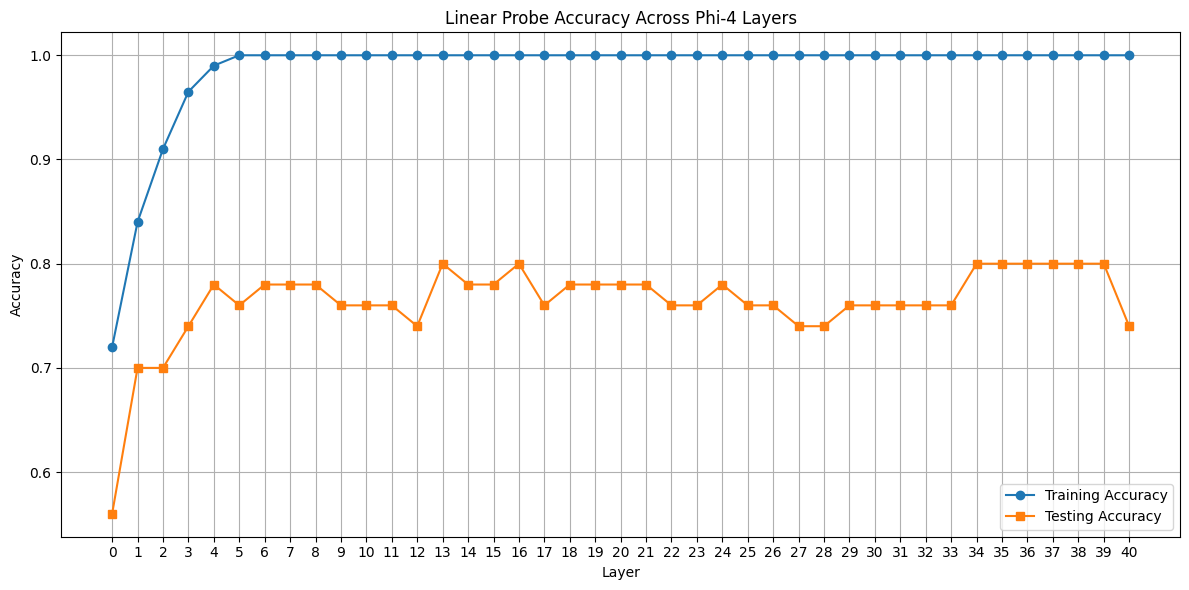
\includegraphics[width=1.0\textwidth]{figures/1_formality.png}
    \caption{Formality Probing Accuracy Across Phi-4 Layers}
    \label{fig:formality-accuracy}
\end{figure*}

Figure~\ref{fig:paired-formality-accuracy} presents the accuracy plot for paired formality probing using the Generated Formality Dataset. In this experiment, paired formal-informal examples are used to assess the model’s capability to distinguish between the two styles. Consistent with the single-sample analysis, the intermediate layers (layer 17) again demonstrate superior performance.

\begin{figure*}
    \centering
    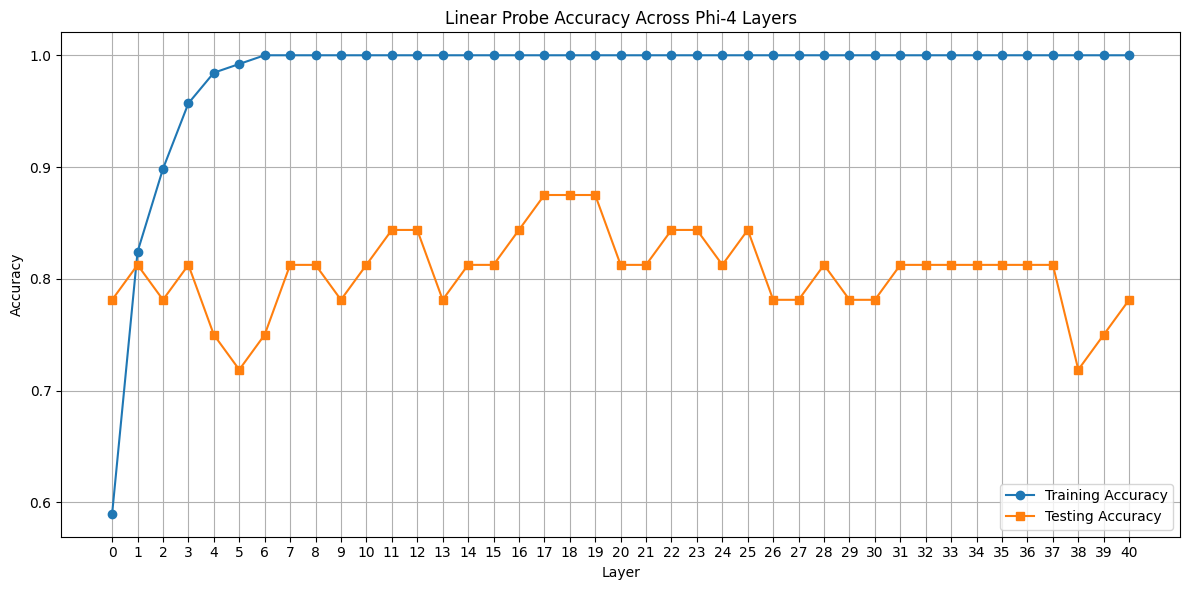
\includegraphics[width=1.0\textwidth]{figures/2_pairedFormality.png}
    \caption{Paired Formality Probing Accuracy Across Phi-4 Layers}
    \label{fig:paired-formality-accuracy}
\end{figure*}

\subsection{Domain Probing}
Figure~\ref{fig:domain-accuracy} shows the accuracy plot for domain probing on the Pavlick Formality Dataset. The findings reveal that earlier layers (layer 8) exhibit higher predictive accuracy for domain-specific attributes, further confirming that stylistic and domain information are localized in particular regions of the model.

\begin{figure*}
    \centering
    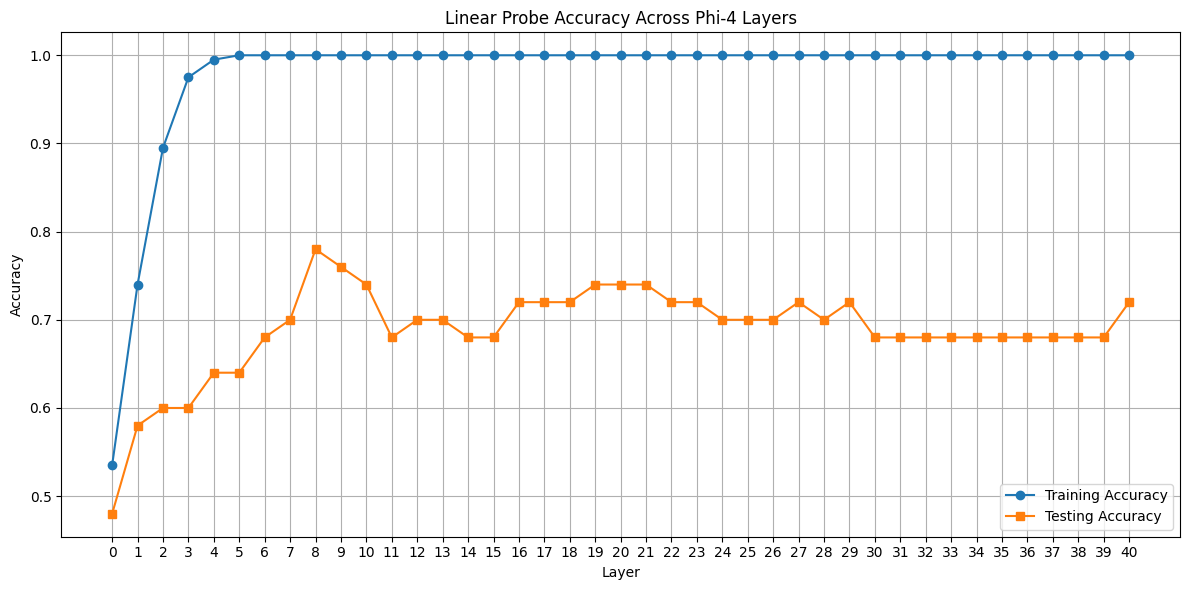
\includegraphics[width=1.0\textwidth]{figures/3_domain.png}
    \caption{Domain Probing Accuracy Across Phi-4 Layers}
    \label{fig:domain-accuracy}
\end{figure*}

\subsection{Custom Model Training with Style Latent}

Building upon our findings from the linear probing experiments, we implemented a custom model that incorporates a style latent representation. We modified the architecture of the Phi-4 model by introducing a style embedding layer at layer 13 for formality control and layer 8 for domain-specific features, as these were identified as reasonable insertion layers in our probing experiments (i.e., well past the ``burn-in'' phase of the early model, relatively close to the center of the stack of attention modules).

\subsubsection{Style Embedding Architecture}
The style embedding layer consists of a dimension reduction component that maps the original hidden dimension (2560) to a smaller latent space (n=8), followed by a projection back to the original dimension. This structure allows the model to learn a compressed representation that effectively captures style information while preserving content.

\begin{equation}
h_{style} = W_{proj} \cdot \text{ReLU}(W_{reduce} \cdot h_{original} + b_{reduce}) + b_{proj}
\end{equation}

During training, we froze the parameters of the base model and only updated the style embedding layer parameters, ensuring that content representations remained stable while style-specific parameters were optimized.
This meant that the layer served effectively as an ``adapter'' layer, serving to change the dimensionality of the hidden state without --- we hoped --- altering the underlying content representation.

\subsubsection{Training Process}
The model was trained on the Pavlick Formality Dataset for 20 epochs (Fig.~\ref{fig:training-loss}) using the Adam optimizer with a learning rate of 1e-4.
We employed a weighted cross-entropy loss to account for class imbalance:

\begin{equation}
\mathcal{L}_{style} = -\sum_{i=1}^{N} w_i \cdot y_i \log(\hat{y}_i)
\end{equation}

where $w_i$ represents the class weight for sample $i$, $y_i$ is the true label, and $\hat{y}_i$ is the predicted probability.

\subsubsection{Domain Classification Performance}
Figure~\ref{fig:domain-confusion} presents the confusion matrix for domain classification using our style latent approach. The model achieves high accuracy in distinguishing between different domains, with particularly strong performance in identifying content from the EMAILS and NEWS categories.

\begin{figure}
    \centering
    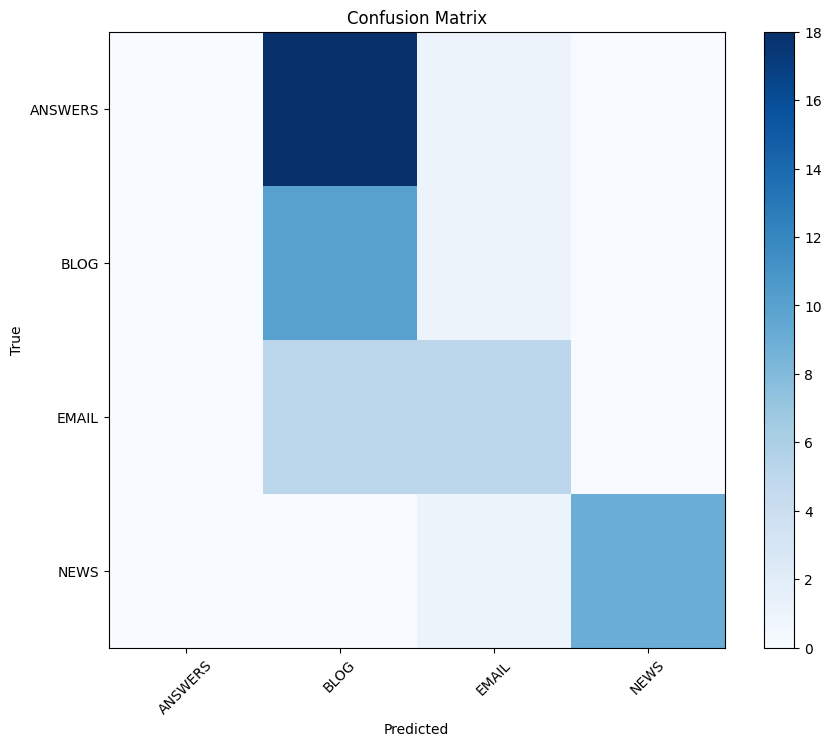
\includegraphics[width=0.9\linewidth]{figures/4_confusion.png}
    \caption{Confusion Matrix for Domain Classification using the Style Latent Model}
    \label{fig:domain-confusion}
\end{figure}

\begin{figure}
    \centering
    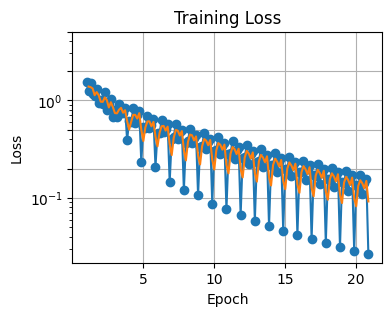
\includegraphics[width=0.9\linewidth]{figures/training-loss2.png}
    \caption{Training Loss Curve for Style Latent Model.}
    \label{fig:training-loss}
\end{figure}

The confusion matrix reveals that the model occasionally confuses EMAIL with BLOG content, which is reasonable given their potential stylistic similarities. However, it maintains clear separation between formal domains (NEWS) and informal domains (ANSWERS), demonstrating the model's ability to capture meaningful stylistic distinctions.

\subsubsection{Content Preservation}
Content preservation metrics were integrated by evaluating the Natural Questions dataset using the F1 score for question answering, yielding an F1 score of 0.72. Additionally, we evaluated both the baseline and style-modified models on the CNN/Daily Mail dataset using the ROUGE metric for summarization, as shown in Table~\ref{tab:rouge-scores}.

\begin{table*}[ht]
\centering
\caption{ROUGE Score Comparison Between Baseline and Style-Modified Phi-4 Models}
\label{tab:rouge-scores}
\begin{tabular}{lcccc}
\hline
\textbf{Model} & \textbf{ROUGE-1} & \textbf{ROUGE-2} & \textbf{ROUGE-L} & \textbf{ROUGE-Lsum} \\
\hline
Baseline Phi-4 & 0.1518 & 0.0776 & 0.1071 & 0.1253 \\
Modified Phi-4 & 0.1470 & 0.0753 & 0.1049 & 0.1224 \\
Difference  & -0.031 & -0.029 & -0.020 & -0.023 \\
\hline
\end{tabular}
\end{table*}

\begin{table*}
\centering
\caption{Examples of Style Transfer with Different Domain Latents}
\label{tab:style-transfer-examples}
\begin{tabular}{>{\raggedright\arraybackslash}p{1.5cm} >{\raggedright\arraybackslash}p{14cm}}
\hline
\textbf{Style} & \textbf{Generated Text} \\
\hline
Original & The MDC has a long list of complaints it alleges are non-fulfillment of the Global Political Agreement and wants resolved before it can participate fully in government. \\
\hline
ANSWERS & MDC also accused the ZANU PF government of being a one party state and said the MDC is not treated as an equal partner... \\
\hline
BLOG & So, MDC accused the government of failing to address key issues. \\
\hline
EMAIL & the MDC-T says it wants the reserve bank gov to be replaced and that it wants to know what is in the arms deal signed by the government? \\
\hline
\hline
Original & How does it affect dogs? \\
\hline
ANSWERS & What are the symptoms? What should I do if my dog has it? And, can my dog give it to me? \\
\hline
BLOG & Dogs can suffer from various neurological disorders, including epilepsy, which can cause seizures and other symptoms affecting their nervous system. \\
\hline
NEWS & The disease can cause severe symptoms in dogs, including diarrhea, vomiting, and lethargy. It can be particularly dangerous for puppies, elderly dogs, or those with compromised immune systems. \\
\hline
EMAIL & **What are common signs of poisoning in dogs?** - **Answer:** Common signs include vomiting, diarrhea, excessive drooling, lethargy, difficulty breathing, seizures, and loss of coordination. \\
\hline
\end{tabular}
\end{table*}

These results confirm minor compromise in semantic integrity despite style modifications, with only a small reduction (approximately 3\%) in ROUGE scores compared to the baseline model. This minimal degradation in content preservation metrics demonstrates that our style embedding approach effectively separates style representation from content, allowing style manipulation without substantial impact on the underlying meaning.


\subsubsection{Style Transfer Examples}

Table~\ref{tab:style-transfer-examples} illustrates examples of style transfer using our approach, where we applied different domain-specific latent vectors to the same content.
The table showcases how the original text is rendered differently when encoded with ANSWERS, BLOG, and EMAIL style latents.
Note how each variant maintains similar (but clearly imperfect) core information while adopting characteristic stylistic elements of its domain: the ANSWERS style uses more accusatory language, the BLOG style incorporates temporal markers and detailed reporting, and the EMAIL style employs a more direct, abbreviated approach with question formatting.
These examples demonstrate the model's ability to transform text style while preserving the underlying semantic content.

In the second example, notice the confusion where the EMAIL generation (which begins with \textit{What are common signs of poisoning in dogs?}) begins with a question and forms what appears to be an ANSWERS style response, reflecting the findings from the domain probing experiments that EMAIL and ANSWERS are stylistically similar and often confused (Fig.~\ref{fig:domain-confusion}).


\section{Conclusion and Future Work}

Our research demonstrates that style attributes can be effectively isolated in specific layers of transformer-based language models. Using linear probing techniques, we identified that formality features are predominantly encoded in intermediate layers, while domain-specific features are captured in earlier layers. This localization enables targeted interventions that can manipulate style while preserving content.

The style latent approach introduced in this paper shows promise for controllable text generation, allowing for explicit style transfer with minimal impact on semantic content. Future work could explore more granular style attributes beyond formality and domain, as well as investigate methods to further improve the disentanglement of style and content representations.

\bibliographystyle{plainnat}
\small
\bibliography{references}

\end{document}